\documentclass[problem]{mcs}

\begin{pcomments}
  \pcomment{MQ_chains_and_antichains_sched}
  \pcomment{format ARM 5/18/15}  
  \pcomment{MISSING FIGURE mq3digraph}
\end{pcomments}

\pkeywords{
  DAG
  schedule
  chain
  antichain
}

\begin{problem} 
Answer the following questions about the dependency DAG shown in
Figure~\ref{fig:dag}.  Assume each node is a task that takes 1 second.

\begin{figure}
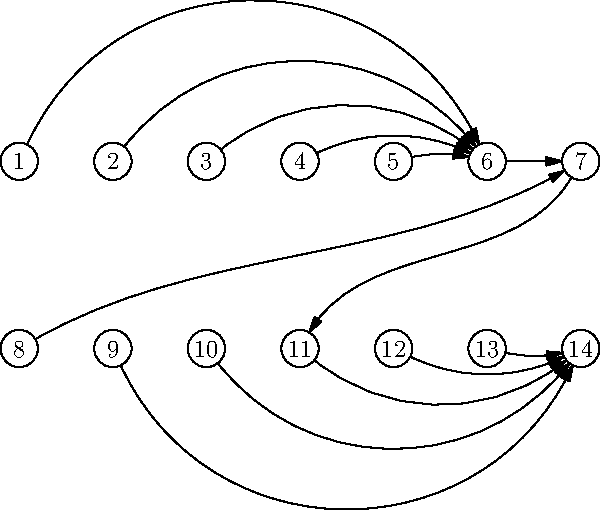
\includegraphics[height=3in]{dag-mq3digraph}
\caption{Task DAG}
\label{fig:dag}
\end{figure}

\bparts

\ppart What is the largest chain in this DAG? If there is more than
one, only give one.

\begin{solution}
One largest chain is $\set{1,6,7,11,14}$.  Greedily computing vertex
depths show that all of the nodes $1,2,3,4,5,8,9,10,12,13$ have depth
$1$, while nodes $6,7,11,14$ have depths $2,3,4,5$ respectively, so
the largest chain has size $5$.
\end{solution}

\examspace[0.4in]

\ppart What is the largest antichain? (Again, give only one if you
find there are more than one). Prove there isn't a larger antichain.

\begin{solution}
One largest antichain is $\set{1,2,3,4,5,8,9,10,12,13}$.  To see that
there isn't a larger one, observe that only one node can be chosen
from the chain $\set{1,6,7,11,14}$, so any antichain must exclude at
least four vertices.
\end{solution}

\examspace[0.4in]

\ppart How much time would be required to complete all the tasks with
a single processor?
\examspace[0.4in]

\begin{solution}
There are 14 nodes, so a single processor would take 14 seconds.
\end{solution}

\ppart How much time would be required to complete all the tasks if
there are unlimited processors available.

\begin{solution}
With unlimited processors, we can take 5 seconds.  This is the length
of the longest chain.
\end{solution}

\examspace[0.4in]

\ppart What is the smallest number of processors that would still
allow completion of all the tasks in optimal time?  Show a schedule
proving it.

\begin{solution}
With 5 processors, we can still finish everyting in 5 seconds. A
schedule showing this is $\set{1,2,3,4,5}$, $\set{6, 8}$, $\set{7}$,
$\set{9,10,11,12,13}$, $\set{14}$.  We cannot do this with fewer than
5 processors because in order to make progress on the longest chain at
every time step, we need to process all of $\set{1,2,3,4,5}$ in step
1.
\end{solution}

\examspace[0.4in]

\iffalse
\begin{solution}
\begin{enumerate}
\item One largest chain is $\set{1,6,7,11,14}$
\item One largest antichain is $\set{1,2,3,4,5,8,9,10,12,13}$
\item There are 14 nodes, so a single processor would take 14 seconds.
\item With unlimited processors, we can take 5 seconds.  This is the length of the longest chain.

\item With 5 processors, we can still finish everyting in 5 seconds. A
  schedule showing this is $\set{1,2,3,4,5}$, $\set{6, 8}$, $\set{7}$,
  $\set{9,10,11,12,13}$, $\set{14}$.  We cannot do this with fewwr
  than 5 processors because in order to make progress on the longest
  chain at every time step, we need to process $\set{1,2,3,4,5}$ in step
  1.
\end{enumerate}
\end{solution}
\fi

\eparts

\end{problem}

\endinput
